\documentclass{report}
\usepackage[margin=1in, paperwidth=8.5in, paperheight=11in]{geometry}
%Math packages%
\usepackage{amsmath}
\usepackage{amsthm}
%Spacing%
\usepackage{setspace}
\onehalfspacing
%Lecture number%
\newcommand{\lectureNum}{7}
%Variables - Date and Course%
\newcommand{\curDate}{January 18, 2017}
\newcommand{\course}{MATH 239}
\newcommand{\instructor}{Luke Postle}
%Defining the example tag%
%\theoremstyle{definition}%
\newtheorem{ex}{Example}[section]
%Setting counter given the lecture number%
\setcounter{chapter}{\lectureNum{}}
%Package for drawing graphs%
\usepackage{tikz}
\usepackage{verbatim}
\usetikzlibrary{arrows}

\begin{document}
%Note title%
\begin{center}
\begin{Large}
\textsc{\course{} | Lecture \lectureNum{}}
\end{Large}
\end{center} 
\noindent \textit{Bartosz Antczak} \hfill
\textit{Instructor: \instructor{}} \hfill
\textit{\curDate{}}
\rule{\textwidth}{0.4pt}

% Actual Notes%
\subsubsection{Review of last lecture}
Let $X$ be a subset of $V(G)$. The \textbf{cut} induced by $X$, denoted by $\delta(X)$, is the set of edges with one end in $X$ and the other not in $X$.\\We also studied a \textbf{theorem} relating connectivity with $\delta(X)$:
\begin{center}
\textit{Graph $G$ is disconnected if and only if there exists a proper, non-empty subset of $X$ of $V(G)$ such that $\delta(X)$ is empty}
\end{center}
We also mentioned three concepts of algorithm analysis:
\begin{itemize}
\item $P$: polynomial time to answer/decide
\item $NP$: polynomial time to convince there exists a solution
\item Co-$NP$: polynomial time to convince there does not exists a solution
\end{itemize}
We also learned about \textbf{trees} and \textbf{forests}:
\begin{itemize}
\item \underline{Tree}: a connected graph containing no cycle
\item \underline{Forest}: a graph (can be either connected or disconnected) containing no cycle
\end{itemize}
\begin{ex}
Some examples of trees
\end{ex}
%Graph 1%
\begin{center}
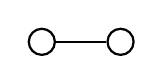
\begin{tikzpicture}[-,auto,node distance=1cm,
                    thick,main node/.style={circle,draw,font=\sffamily\small}]
  %C_4%
  \node[main node] (1) {};
  \node[main node] (2) [right of=1] {};
    
  \path[every node/.style={font=\sffamily\small}]
    (1) edge node [left] {} (2);
\end{tikzpicture}$\qquad\qquad$
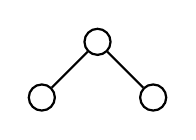
\begin{tikzpicture}[-,auto,node distance=1cm,
                    thick,main node/.style={circle,draw,font=\sffamily\small}]
  %C_4%
  \node[main node] (1) {};
  \node[main node] (2) [below right of=1] {};
  \node[main node] (3) [below left of=1] {};    
  
  \path[every node/.style={font=\sffamily\small}]
    (1) edge node [left] {} (2)
    	edge (3);
\end{tikzpicture}$\qquad\qquad$
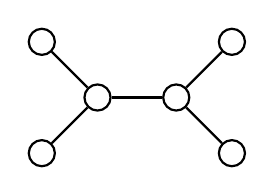
\begin{tikzpicture}[-,auto,node distance=1cm,
                    thick,main node/.style={circle,draw,font=\sffamily\small}]
  %C_4%
  \node[main node] (1) {};
  \node[main node] (2) [right of=1] {};
  \node[main node] (3) [above left of=1] {};    
  \node[main node] (4) [below left of=1] {}; 
  \node[main node] (5) [above right of=2] {}; 
  \node[main node] (6) [below right of=2] {}; 
    
  \path[every node/.style={font=\sffamily\small}]
    (1) edge node [left] {} (2)
    	edge (3)
    	edge (4)
    (2) edge (5)
    	edge(6);
\end{tikzpicture}
\end{center}
The question we'll focus on today is \textit{how can I convince you that a tree doesn't contain a cycle?}
\section{More on Trees and Forests}
\subsection{Leaves}
A \textbf{leaf} is a vertex of degree one.
\subsubsection{Theorem 7.1.1:}
\begin{center}
\textit{If $T$ is a tree with at least two vertices, then $T$ has a leaf}
\end{center}
\textbf{Proof of Theorem 7.1.1:} to prove this theorem, we'll instead prove the following (it will end up proving that $T$ will have at least \textit{two} leaves):
\begin{center}
\textit{If $G$ has a minimum degree of at least 2, then $G$ contains a cycle}
\end{center}
\textbf{Proof:} Let $P = v_0v_1 \cdots v_k$ be a longest path in $G$. Since $G$ has minimum degree of at least 2, then $v_0$ has at least two neighbours (one of which is $v_1$). Thus, there exists a neighbour $u$ of $v_0$ distinct from $v_1$.\\
If $u \in V(P)$, say $u = v_i$, then $C = v_0v_1, \cdots, v_iv_0$ is a cycle of $G$, as desired.\\
Now suppose  $u \notin V(P)$, but then $P^\prime = uv_0v_1\cdots v_k$ is a path that is longer than $P$, a contradiction.\\
Now, let's prove
\begin{center}
\textit{If $T$ is a tree with at least two vertices, then $T$ has at least two leaves}
\end{center}
\textbf{Proof:} Let $P = v_0v_1 \cdots v_k$ be a longest path. Note that $k \geq 1$ because $T$ is connected with at lesat two vertices. Now $v_0$ does not have a neighbour $u \neq v_i$, for if $u \notin V(P)$, then $p^\prime - uv_0v_1 \cdots v_k$ is a longer path, a contradiction.\\
If $u \in V(P)$, say $u = v_i$, $C = v_0v_1, \cdots, v_1v_0$ is a cycle, contradicting that it's a tree.\\
So $v_0$ has degree one (i.e., is a leaf). But by symmetry, $v_k$ is also a leaf, and since $k \geq 1$, $v_0 \neq v_k$, so $T$ has at least two leaves, as desired.
\subsubsection{Theorem 7.1.2:}
\begin{center}
\textit{If $T$ is a tree and $v$ is a leaf of $T$, then $T-v$ is a tree}
\end{center}
\textbf{Proof of Theorem 7.1.2:} $T-v$ is a forest, because $T-v$ is a subgraph of $T$, and every subgraph of a forest is a forest ($T$ is a tree, but by definition, it's a forest too).\\
Now we want to claim $T-v$ is connected and hence a tree. To see this, let $x, y \in V(T)-v$. Since $T$ is connected, there exists a path $P$ from $x$ to $y$ in $T$. Note that $v$  is \underline{not} in $P$ because $v$ has degree one and is not an end of $P$. But then $P$ s a path from $x$ to $y$ in $T-v$, so $T-v$ is connected, as desired.
\subsubsection{Corollary}
\begin{center}
\textit{$T$ is a tree if and only if there exists a sequence of vertices $v_1,v_2,\cdots,v_{n-1}$ such that if $T_i = T - \{v_1,v_2,\cdots,v_{n-1}\}$, then $T_i$ is a tree}
\end{center}
This shows that deciding if $G$ is a tree is in $NP$.
\subsubsection{Algorithm for Deciding if G is a Tree}
From the proven theorems shown above, we can create an algorithm for determining if $G$ is a tree:
\begin{itemize}
\item If $\vert V(G) \vert = 1$, then yes!
\item If $\vert V(G) \vert \geq 1$, determine if $G$ has a leaf:
\begin{itemize}
\item If yes, delete the leaf $v$ and recurse on $G-v$
\item If no, then no!
\end{itemize}
\end{itemize}
This means that deciding if $G$ is a tree is in polynomial time.
\subsubsection{Theorem 7.1.3:}
\begin{center}
\textit{If $T$ is a tree, then $\vert E(G) \vert = \vert V(G) \vert - 1$}
\end{center}
\textbf{Proof of Theorem 7.1.3:} Proceed by induction on $\vert V(T) \vert$:\\
\textit{Base case:} If $\vert V(T) \vert = 1$, then $\vert E(G) \vert = 0$, as desired.\\
\textit{Inductive case:} If $\vert V(G) \vert \geq 2$, then $T$ has a leaf $v$, by our earlier theorem. by previous theorem, $T-v$ is a tree.
By induction, $\vert E(T-v)\vert = \vert V(T-v)\vert - 1$. However, $|V(T)| = |V(T-v)| + 1$, and $\vert E(T)\vert = \vert E(T-v)\vert + 1$, since v has degree one. Thus, $\vert E(G) \vert = \vert V(G) \vert - 1$, as desired.
%END%
\end{document}